\section{Основная часть}
    \subsection{Постановка задачи}
        Пусть даны известные квадратная матрица $A$, вектор $f$ и неизвестный вектор $x$ размерностями $n$. Нужно найти вектор $x$ в матричном уравнении $Ax = f$, используя метод отражений.
        
    \subsection{Описание алгоритма}
        Метод отражений состоит в выполнении $(n-1)$ шагов, в результате чего матрица $A$ приводится к верхней треугольной форме и в последующей решении системы с такой матрицей.

        Для этого на каждом шаге $k$ будем находить вектор нормали $p$, характеризующий ортогональную матрицу отражения $P$, которая обнулит все поддиагональные элементы $k$-того столбца.

        Обозначим вектор нормали и матрицу на шаге $k$: $p^{(k)}, A_{k} = \left( a_{ij}^{(k)} \right)$, тогда
        \[
            p_k^{(k)} = a_{kk}^{(k-1)} + \sigma_k \sqrt{\sum_{l=k}^{n} \left( a_{lk}^{(k-1)} \right)^2 }, \quad \sigma_k = \left\{
                \begin{matrix}
                    1, & a_{kk}^{(k-1)} \geq 0, \\
                    -1, & a_{kk}^{(k-1)} \leq 0,
                \end{matrix}
            \right.
        \]
        \[
            p_i^{(k)} = 0, \quad i = 0, \dots, k - 1; \qquad p_i^{(k)} = a_{ik}^{(k-1)} , \quad i = k+1, \dots, n;
        \]
        Определение матрицы $ P_k = I - \frac{2 p^{(k)} \left(p^{(k)}\right)^*}{(p^{(k)},p^{(k)})}$. Будем применять данную матрицу с обоих сторон уравнения. Связь шагов $ A_k = P_k A_{k-1},~ f^{(k)} = P_k f^{(k-1)} $.Запишем явные формулы элементов матрицы $ A_k $ и вектора $ f^{(k)} $:
        \[
            a_{kk}^{(k)} = - \sigma_k \sqrt{\sum_{l=k}^{n} \left( a_{lk}^{(k-1)} \right)^2 }, \quad
            a_{ij}^{(k)} = a_{ij}^{(k-1)} - 2 p_i^{(k)} ~\frac{\sum\limits_{l=k}^{n} \left( p_l^{(k)} a_{lj}^{(k-1)} \right)}{\sum\limits_{l=k}^{n} \left( p_{l}^{(k)} \right)^2},
        \]
        \[
            f_i^{(k)} = f_i^{(k-1)} - 2 p_i^{(k)} ~\frac{\sum\limits_{l=k}^{n} \left( p_l^{(k)} f_l^{(k-1)} \right)}{\sum\limits_{l=k}^{n} \left( p_{l}^{(k)} \right)^2}; \quad
            i = k, \dots, n, \quad j = k+1, \dots, n.
        \]

        В результате выполнения всех $(n-1)$ шагов получится система $ A_{n-1} x = f^{(n-1)} $, где матрица $ A_{n-1} $ является верхней треугольной, поэтому вектор $ x $ можно найти последовательно снизу вверх:
        \[
            x_n = \frac{ f_n^{(n-1)} }{ a_{nn}^{(n-1)} }, \quad x_i = \frac{ f_i^{(n-1)} - \sum\limits_{j=i+1}^n a_{ij}^{(n-1)} x_j  }{ a_{ii}^{(n-1)} }, \quad
            i = n-1, \dots, 1.
        \]

    \subsection{Описание тестов, использованных для отладки}
        Для тестирования были использованы данные:
        \[
            A = \left(
                \begin{matrix}
                    10.9 & 1.2 & 2.1 & 0.9 \\
                    1.2 & 11.2 & 1.5 & 2.5 \\
                    2.1 & 1.5 & 9.8 & 1.3 \\
                    0.9 & 2.5 & 1.3 & 12.1
                \end{matrix}
            \right), \quad
            f = \left(
                \begin{matrix}
                    -7. \\
                    5.3 \\
                    10.3 \\
                    24.6
                \end{matrix}
            \right), \quad
            x = \left(
                \begin{matrix}
                    -1 \\
                    0 \\
                    1 \\
                    2
                \end{matrix}
            \right)
        \]


    \subsection{Вычислительные эксперименты}


        \subsubsection{Анализ погрешностей приближённых решений}


    \subsection{Оценка количества арифметических операций}
        Оценим количество арифметических операций метода отражений:
            \begin{enumerate}
                \item Почти во всех формулах используется сумма $\sum_{l=k}^{n}$, которая использует $(n-k)$ операций сложения, что в итоге даёт $\frac{n(n-1)}{2}$ операций сложения и всех операций внутри суммы.
                \item Для вычисления $k$-того элемента вектора $p$ во всем методе используется $n-1 + \frac{n(n-1)}{2}$ операций сложения и столько же умножения, а также $ n $ операций вычисления корня.
                \item Для вычисления матрицы $A$. 
            \end{enumerate}


    \subsection{Оценка временных ресурсов}


    \subsection{Проверка}


    \subsection{Доп}




% \begin{figure}[H]
%     \centering
%     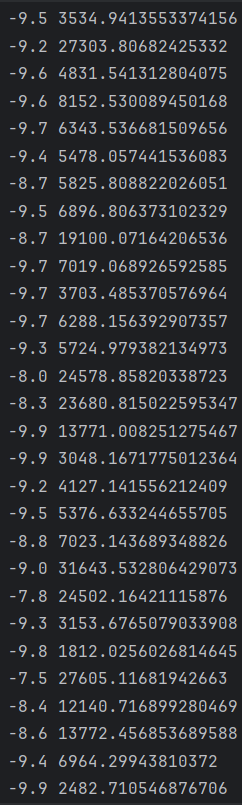
\includegraphics[width=6cm]{pictures/BigConditions.png}
%     \caption{Log10 разности и число обусловленности решений, которые не превысили точность $10^{-10}$.}
% \end{figure}